% !TEX root = ../report.tex

\chapter{Software}\label{software}
The software architecture was centred on the event driven implicit implication
design pattern~\cite{garlan1993introduction}. This architecture design pattern is
also known as the ``Hollywood'' design pattern due to its definition of ``Don't
call us, we'll call you''. With regards to software architecture this means
modules are signalled to start by other modules and this is propagated through
the system with ``events'' triggering other ``events'' within the system.

To implement this architecture, each part of the system can be defined as its own
module with a function which triggers its invocation and a function which can
broadcast events if required. A methodology for implementation of this system is
the publish/subscribe model. Each modules' invoking function is a publisher and
modules which would be triggered by this function are known as subscribers. Using
this method in the context of this project, means the software has strong support
for reuse---as new sensors or libraries can be plugged in and subscribe to the
appropriate events---and loose coupling throughout the system means that
maintenance of each module can take place independently.

In robotic systems, this architecture is highly beneficial as each of the sensor
and actuator systems can run independently publishing their data for feedback,
using event driven implicit invocation through data driven programming. This
reduces the risk of system crashes as module crashes are isolated, improving
robustness.

\section{ROS}\label{soft/ROS}
In order to implement this architecture, and following extensive research(see
Section~\ref{litreview/ROS}, the Robot Operating System (ROS) library was
selected as a framework. The ROS library makes it simple to design and implement
individual modules within a system and uses a central control node named
``roscore'' to manage publish and subscribe ``topics'' between modules.

\subsection{Design}\label{soft/ROS/design}
Following the decision to use ROS to implement our chosen architecture, a modular
approach was adopted for the design of each of the components within the system~
\ref{elec}. Hence, a system block diagram was developed to visualise data flow
within the system. \todo{put in block diagram} The block diagram in Figure~
\ref{BlockDiagram} demonstrates the modularisation of the system and also the
expectation that the AI module at the top of the system will be completely
independent from the other components of the system. By making the control module
an API, AI algorithms can be interchanged easily for testing. The modular
approach also means sensor and actuator modules can be plugged in and out as
desired and could easily be changed if needed at any point in the project.

Each module can be programmed in a different language before being converted to a
ROS node, which publishes and subscribes, using the appropriate methods for that
language. Although the majority of the system will be programmed in Python,
allowing different programming languages means that timing or processing
sensitive operations can be programmed in C or C++ as required. Once converted to
a ROS node, each module can then be started individually using a ROS launch file.
Launch files are used by ROS to create and start a number of nodes within a
system with any number of parameters. Again, due to the modular approach and use
of ROS, launch files allow various configurations of modules to be tested easily.

In order for ROS launch files to function, the directory structure within the
``catkin''~\cite{catkin} workspace must be configured correctly. ``Catkin is the
CMake based build system that is used to build packages in ROS''~\cite{gitcatkin}
and requires a strict directory structure in order to build each of the
individual modules within the project. Packages within ROS allow code to be
maintained and compartmentalised, and by using packages throughout existing
packages can be added easily.

Considerations of appropriate packages were made and a final design UML diagram
created\todo{UML~\ref{UMLDiagram}}. This demonstrates a full system
implementation and the expected interactions between each of the modules within
the program.


\subsection{Implementation}\label{soft/ROS/impl}
In order to enable rapid development of the system, the ROS packages were
primarily written in Python, with the \verb|rospy| library used to
interface with ROS functionality.

Each of the individual modules discussed in Section~\ref{elec} was
implemented as a ROS node, generally encapsulated in a single Python
script. In order to adhere to best practices and ensure consistency across
the code base, each node was represented as class, with an
\verb|__init__()| method initialising the node and a \verb|spin()| method
which is called to run the node's main loop. In nodes which perform
recurring work, such as polling sensors for data, this method uses a
\verb|rospy.Rate| object to schedule tasks, whereas nodes that respond to
events on subscribed topics simply call \verb|rospy.spin()|, which
prevents the script from exiting until a ROS shutdown signal is received.

The \verb|rospy.Publisher| class is used to publish messages of a pre-
determined type to a topic with a given name. Similarly,
\verb|rospy.Subscriber| is used by nodes wishing to listen for messages on
a specific topic. The constructor of this class specifies a callback
function, which takes the message as a parameter. By loading parameterised
values at startup, the code maintains flexibility, as different values can
be used in launch files for different applications.

Listing~\ref{lst:ros_node} shows an example of a ROS node that publishes
at a predefined rate. The rate can be passed to the node as a parameter in
the launch file, and in this case defaults to \SI{10}{\Hz}. The data is
set by a callback method, which is called by a subscriber to another
topic. In general, callback methods were kept very short in order to
prevent blocking of the subscriber's thread, with any processor-intensive
work executed in the main loop.

\begin{lstlisting}[caption={Example ROS node}, label={lst:ros_node}]
#!/usr/bin/env python
import rospy
from std_msgs.msg import Int16


class Node:
    def __init__(self):
        rospy.init_node('node_name')
        self.rate = rospy.Rate(rospy.get_param("~rate", 10))
        rospy.Subscriber('topic1', Int16, self._callback)
        self.pub = rospy.Publisher('topic2', Int16, queue_size=10)
        self.data = 0

    def spin(self):
        try:
            while not rospy.is_shutdown():
                self.pub.publish(self.data)
                self.rate.sleep()
        finally:
            self._cleanup()

    def _callback(self, msg):
        self.data = msg.data

    def _cleanup(self):
        # Perform cleanup operations such as saving data to files
        # or clearing GPIO pin configuration
        pass


if __name__ == '__main__':
    try:
        node = Node()
        node.spin()
    except rospy.ROSInterruptException:
        pass
\end{lstlisting}


\subsubsection{Python version}
This project currently uses Python 2.7, which will no longer be supported
after January 2020~\cite{python2-eol}. The reason for this choice was the
lack of official support for Python 3.x in ROS Kinetic. While it is
possible to use Python 3 with ROS, various issues may arise resulting from
incompatibility~\cite{medium-ros-python3}. In the interest of stability,
it was decided to use the older version. Migration to ROS 2, which is
currently under heavy development but will have native support for Python
3, is recommended in future~\cite{ros2}.

\subsection{Testing}\label{soft/ROS/test}
In addition to each of the nodes being tested independently in a similar
manner to how each of them were tested in isolation throughout the~\ref{elec}
Section, the nodes were tested in a number of different
configurations.
\todo{David maybe needs to write this}

Each of the topics can be tracked from the main graph of nodes in the ROS
runtime using the command $rqt graph$. This produces the following output,
\todo{put rqt graph of nodes and topics in here and dicuss}.


\subsection{Deployment}\label{soft/ROS/deploy}
Since system testing was closely tied to the hardware of the robot, the
ability to rapidly deploy changes to the robot was crucial to the
development process. To this end, a shell script (\verb|deploy.sh|) was
written to copy any changes to robots connected to the network. The script
uses \verb|rsync| to copy any modified source or configuration files in
the Catkin workspace, and fetches any output files generated by previous
executions of the code. Since the Raspberry Pis are unable to retain
system time between boot cycles, and \verb|rsync| relies on system time to
detect file modifications, the script additionally syncs the system time
of the Pi to the host machine. The system time is set using UTC in order
to prevent problems caused by time zones and daylight saving time.

The installation of software dependencies proved to be less trivial due to
difficulties connecting to the internet and WANET simultaneously.
Dependencies were initially installed manually on a single Pi connected to
the internet, and were then transferred to the other robots by copying an
image of the SD card. This method had the additional benefit of ensuring
that all Pis were running the same versions of any dependencies.

\section{Communication}\label{soft/comms}
The communication node's requirements were to allow the agents to
be able to send and receive messages to each other. The structure
of these messages should allow for any object to be able to be sent
regardless of the data types, depth or complexity of the objects.
Each robot should also be able to simultaneously be listening for
incoming messages whilst sending messages to a different robot.
With the aim of allowing scalability, the communication system
should be able to handle robots listening to multiple robots at the
same time, whilst also being connected to send messages to different
robots at the same time.

The communication system also requires a network or communication
technology to allow all of the robots in the system to be able to
communicate with each other. Each of the robot's will also require
a unique identifier to allow sending messages to specific robots
rather than broadcasting all messages to all robots.

\subsection{Design}\label{soft/comms/design}
In order to implement these requirements the first decision was the
method the robots were going to use to communicate. A few options
for this were considered such as Bluetooth and WiFi. After
researching  and considering these options, we initially decided to
use a Wireless Ad-hoc Network (WANET).

WANET is a wireless network where the nodes can be located anywhere
globally and does not require any infrastructure such as a router or
mobile network. The underlying design is such that the nodes believe
they are part of a single-hop or multiple-hop wireless network at the
physical layer and the data link layer as part of the MAC sublayer~
\cite{rajesh2015congestion}. The wireless channels are often shared
and so use carrier sense multiple access protocols to handle multiple
nodes attempting to use the channel at the same time. This is known
as link-level congestion and increases packet service time,
decreasing utilization and overall throughput. Although scalability
is an important  factor, it was deemed that WANET's handling of
congestion was sufficient given the anticipated level of
communication across the system at any time would be low.

Each node in the WANET is assigned a local IP address.
Anything that connects to the network can then send messages through
the network provided it knows this address. As a result, a robot
needs a way to find this address if it knows who it wishes to send
a message to. The simplest method for this is to use a lookup table
that maps the robot's name to their fixed IP in the network, allowing
all nodes in the network access to this.

After deciding to use WANET, a decision  had to be made in how to format
the data to send over the network. A few options were available such as
using JSON, XML or a custom-structure. It was decided the best option was
to use JavaScript Object Notation (JSON) objects after consultation with
Dr~Irvine as discussed in Section~\ref{pm/consultations}. JSON is a
standard data-interchange format that is easy for humans to read and write
as it uses attribute-value pairs and array data types.

For the structure of the communication module after considering various options,
a client-server system was decided upon. The client is the node
responsible for sending the messages whilst the server is responsible
for listening for incoming messages. As these would be separate nodes,
these would work independently of each other and so would allow for the
robot to send and receive messages simultaneously.

\subsection{Implementation}\label{soft/comms/impl}
Look-up table
First copy of send/receive that caused multi-message issues
The new implementation with the thread-safe code

To implement these requirements a $comms.py$ file was created which contain
the function definitions and address lookup table that the ROS server and
client nodes would use to communicate. Firstly a python dictionary of the
robot's IP addresses as well as our laptop for testing purposes was created.
A $lookupIP(name)$ function and a $lookupname(ip)$ function were created for
readability and maintainability. Secondly, a function were needed that could
create the JSON message ($tojsn()$) and one that could extract the data from
the message ($fromjson()$).

\begin{lstlisting}
def tojson(host_ip, hostname, data):
    # receiver ip and hostname, our ip and hostname, classname
    sender_ip = socket.gethostbyname(socket.gethostname())
    header = [host_ip, hostname, sender_ip,
    Address_lookup.lookupname(sender_ip), type(data).__name__]
    content = [header, data]
    message = json.dump(content, separators=(',', ':'))
    return message

def fromjson(packet):
    message = json.loads(packet)
    try:
        target = message[0][0]
        if target == socket.gethostbyname(socket.gethostname()):
            return message[1]
        else:
            return -1
    except IndexError:
        return -2
\end{lstlisting}
The header created includes the IP and name of both the sender and the
receiver as well as the type of python object the data is. The header along
with the data to be sent is converted to JSON and returned as a string. When  converting from JSON it checks that it was the intended recipient of the
message, returning $-1$ to indicate it was not, before returning the data
object located at index 1 (header is index 0). These are the four helper
methods used by the send and listen methods.

In order to physically send and receive the data the Python Socket library
is used. This interface's $sockett()$ function returns a socket object whose
methods implement the Unix socket system calls.
\begin{lstlisting}
# data is python object to send
def send(hostname, data):
    host_ip = lookupip(hostname) # The remote host
    port_number = 8001 # The same port as used by the server
    message = tojson(host_ip, hostname, data)
    s = socket.socket(socket.AF_INET, socket.SOCK_STREAM)
    if not s.connect_ex((host_ip, port_number)):
        s.sendall(message) # Sends string (of JSON)
        s.close()
\end{lstlisting}
The send function looks up the IP of the destination and gets the JSON object
of the message. It then attempts to connect using the $connect_ex()$ which
returns 0 if successful. If so then it can use the socket methods to send the
data and then close the connection.

\begin{lstlisting}
def listen():
    PORT = 8001 # Arbitrary non-privileged port
    s = socket.socket(socket.AF_INET, socket.SOCK_STREAM)
    s.bind(('0.0.0.0', PORT))
    s.listen(2)
    conn, addr = s.accept()
    packets = ''
    while 1:
        packet = conn.recv(1024)
        if not packet:
            break
        packets += packet
    conn.close()
    message = fromjson(packets)
    return message
\end{lstlisting}
When listening for incoming messages, the created socket object must bind to
an IP address and port number. The address of 0.0.0.0 results in it listening
to any incoming messages. The $listen()$ function starts the node listening
whilst setting the number of queued connections allowed. In this case it is
set to 2 but can be increased when scaling the system to use many more agents.
Once the socket  accepts a connection, we can continually store the packets
until no more data is received. After which the connection can be closed and
the data read from the JSON strings and returned.

This implementation was set up and initially tested between a laptop and a Pi
by remotely connecting to the Pi. When this succeeded in sending multiple
messages between them, we remotely connected to another Pi and attempted to
have them send messages back and forth to each other. Again this was successful
and so this demonstrated the basic functionality of the communication system was
working.

When undertaking more extensive testing, an important issue with the previous
code was found. When nodes were sending messages to each other simultaneously
at least one of the nodes would fail. For example, if robot A sends a message to
robot B but before the message has finished sending, robot B sends a message to
robot A then the receiver of robot B crashes and robot A never receives the message.
If robot B were to send to a third robot, C, then robot B's receiver would still
fail as would one of either robot B or C.

As a result of this bug, the implementation would have to be changed to handle
multiple connections properly. Various potential solutions were discussed,
such as using multiple ports so as not to kill the socket connection when
attempting to connect again or to use a multi-connection selector as part of
the server to handle multiple requests \cite{multiconnectionServer}.
Alternatively, if the server can always be listening for incoming messages by
utilising multiple threads then there would be no downtime of the system and
thus each message would be successfully sent. As a result, we choose to
design a thread-safe version of the existing code base.

This was implemented by defining ThreadedTCPServer and ThreadedTCPRequestHandler
classes to be used by the listener as shown in SocketServer documentation~\cite{socketServerDocs}.
\begin{lstlisting}
class ThreadedTCPRequestHandler(SocketServer.BaseRequestHandler):
    def messageHandler(self, x):
        print x

    def handle(self):
        data = self.request.recv(1024)
        message = fromjson(data)
        self.messageHandler(message)

class ThreadedTCPServer(SocketServer.ThreadingMixIn, SocketServer.TCPServer):
    pass
\end{lstlisting}
The $listen()$ function is changed to take in a handler parameter. This is
passed a function which is used instead of the messageHandler function in
the ThreadedTCPRequetHandler before it is used to create a ThreadedTCPServer
object as shown.
\begin{lstlisting}
def listen(handler):
    ThreadedTCPRequestHandler.messageHandler = handler
    HOST, PORT = "0.0.0.0", 8001
    server = ThreadedTCPServer((HOST, PORT), ThreadedTCPRequestHandler)
    ip, port = server.server_address
    # Start a thread with the server -- that thread will then start one
    # more thread for each request
    server_thread = threading.Thread(target=server.serve_forever)
    # Exit the server thread when the main thread terminates
    server_thread.daemon = True
    server_thread.start()
    return server
\end{lstlisting}
The handler object passed is a function that will solely publish the
message contents so the relevant subscribers can use the data received
from the other agent. As a new thread is being created for each request
there should be no node crashes from having the process interrupted as
it will be happening on a different thread.
\todo{Is testing for just the final designed testing - cause this goes impl - testing  impl - testing and not sure how we want to handle that. All writing is here just where the heading goes?}

\subsection{Testing}\label{soft/comms/test}

In order to test this version it was important to first ensure that the
working functionality from the previous version still worked. Therefore
the same initial tests were applied to this implementation which passed
as expected. In order to test whether this was thread-safe, a number of
tests were executed. The first test involved creating a loop that would
send 100 messages from robot A to robot B. When this succeeded without any
node crashes, the test was repeat but with robot B sending messages to robot A
simultaneously. This previously would have crashed the nodes but with the
server's listening on separate threads for each request, this was handled
successfully. This test was repeated with robot B sending messages to robot C
instead of robot B. This too was successful with the messages being received
without any being lost. The test was repeated but the limit on the number of
messages being send was removed, and so the messages would, in theory,
continue to create new threads to listen to the incoming messages. This
worked initially, but due to there being no delay in between sending messages,
thousands of threads were being created quickly. This resulted in the node
crashing as the thread limit had been reached, however, this happened after
over 50 thousand messages in quick succession (due to no delay). As a result,
this was determined to be the upper limit of this system, that with this set
up would never be close to reached and so it was determined that the system
was sufficiently thread-safe to be used.

\section{PID Controller}\label{soft/PID}
The PID controller uses feedback from the encoders to maintain 
a straight line of movement and maintain each of wheels at a constant 
velocity. The PID controller is a feedback loop which is designed to 
eliminate errors in the actuator systems by the mathematical description 
(see Equation~\ref{eqn:pid}). By tuning $ K_p $, $ K_i $ and $ K_d $ for 
the system in question, the error in the system can be reduced. 

\subsection{Design}\label{soft/PID/design}
The PID controller of the system was handled by an external library --- 
``differential-drive''~\cite{diffdrivelib}. The library is specifically 
designed for differential drive robots and takes a ROS twist message
\todo{~\cite{}Twist Message}, converting this to a motor command for each 
motor. It then uses the feedback from the encoders to monitor the movement 
of the wheels and adjust future motor commands accordingly, in an attempt 
to maintain a straight line of movement. The library has a number of nodes 
which each  carry out different tasks within the motor control of the 
system. The library has the parameters $ K_p $, $ K_i $ and $ K_d $ to 
tune the PID appropriately. 

In addition to this, the library has a simulator node named ``wheel-
loopback'' which can be used to simulate the movement of wheels and also 
therefore to tune the PID. Although the PID tuning parameters would be 
different in practise as the weight, inertia and torque of the robot are 
contributing factors, methodologies for tuning the PID were tested using 
the simulation. The various methods discussed (see Section~\ref{litreview/
robotics/pid} were attempted and outcomes recorded. 

\subsection{Ziegler-Nichols}\label{soft/PID/zn}
As most of the research carried out pointed towards the Ziegler-Nichols 
method being an effective way of tuning PID, this was tried first directly 
on the robot. In order to tune the PID in real time, the values of $ K_p 
$, $ K_i $ and $ K_d $ were published to the ROS system from a terminal 
while ``roscore'' was running. $K_p$ was increased until oscillations were 
seen in the system --- the determination of an oscillation was vaguely 
defined across literature and hence this was done by eye --- and this was 
set as the critical gain of the system $K_u$. The period of oscillation 
$T_u$ was then measured from $K_u$. From these values, a tuning table~
\cite{mccormack1998rule} of tuning rules was used to calculate values for 
$K_p$, $ K_i $ and $ K_d $.  This was carried out with the results shown 
in Table~\ref{zn_pid_tuning}.

\begin{table}[!ht]\centering
\caption{Ziegler-Nichols PID Tuning
\label{zn_pid_tuning}
    \begin{tabular}{ccc}
        \toprule
        \thead{method} & \thead{$K_u$} & \thead{$T_u$[\si{\second}]} & \thead{$K_p$} & \thead{$K_i$} & & \thead{$K_d$}\\
        \midrule
		ZN & 775 & 0.14 & 465 & 6642 & 8.13\\
		ZN & 800 & 0.14 & 480 & 6857 & 8.4\\
		NO-OV & 775 & 0.14 & 155 & 2214 & 7.49\\
		NO-OV & 800 & 0.14 & 160 & 2240 & 7.47\\ 
        \bottomrule
    \end{tabular}
\end{table}

In practice, these values for $K_p$, $ K_i $ and $ K_d $ were not accurate 
and produced an aggressive stop-start motion in the movement of the robot. 
This was due to these methods providing an aggressive gain and overshoot 
which resulted in the motors being run at high speed followed quickly by 
low speed to average the correct speed. Due to the high current drawn by 
the motors when stopping and starting this was not suitable for this 
project's application. 


\subsection{Manual}\label{soft/PID/man}
Due to the high current spikes during testing of these methods, batteries 
were being drained rapidly and hence, the library simulation was used to 
find a usable tuning method. A more practical solution was found~
\cite{practicalPID}, which approached the problem without calculating 
values. Using the simulation and output graphs --- obtained using the ROS 
function \verb|rqt_graph| --- to determine correct behaviour, $K_p$ was 
increased until the system oscillated. $K_p$ was then halved and $K_i$ 
introduced to increase the rate of change in the system\todo{???}. $K_d$ 
could then be slowly increased to minimise the overshoot in the system. 
Following one iteration of this process the velocity scaling was reduced 
and the process repeated. The results are shown in Table~\ref{

\begin{table}[!ht]\centering
\caption{Manual PID 
\label{manual_pid_tuning}
    \begin{tabular}{ccc}
        \toprule
        \thead{method} & \thead{$K_p$} & \thead{$K_i$} & & \thead{$K_d$}\\
        \midrule
		Before Velocity Scaling & 102.5 & 2.5 & 0.88\\
		After Velocity Scaling & 0.2775 & 0.0075 & 0.007\\
        \bottomrule
    \end{tabular}
\end{table}

These values resulted in far less aggressive motion in the movement of the 
robot. Despite this, current spikes still occurred and following a 
consultation with Dr Gordon Dobie (see Section~\ref{pm/consultations}) a 
rate control implementation (see Section~\ref{litreview/robotics/
ratecontrol}) was used. Values for this were tuned slightly from the 
manual values determined after velocity scaling resulting in $K_p = 0.176$ 
and $K_d = 0.008$. As rate control does not turn off the motors completely 
when overshoot occurs --- instead using a change in rate to control the 
motor velocity --- no $K_i$ term is required. This was tested and results 
in significantly less aggressive motion of the robot and a far straighter 
line of motion. 


\section{Odometry Sensor Fusion}\label{soft/odometry}

\subsection{Wheel Odometry}\label{soft/odometry/design}

Wheel Odometry is derived in two parts. Firstly, the speed


\subsection{IMU}\label{soft/odometry/imu}

As was discussed in Section~\ref{elec/imu}, the IMU can also be used to 
perform dead reckoning, and this can be fused with the wheel odometry to 
improve the accuracy of the system.

For other nodes to use the IMU data, the readings had to be converted into 
a ROS IMU message~\cite{ROSIMUMsg} consisting of: a ROS header message~
\cite{ROSHeaderMsg}; a quaternion representing the orientation; a 3 
element vector for the rotational speed; a 3 element vector for the linear 
acceleration; and covariance matrices for each of these measurements. The 
code imu\_node uses to create an IMU messages is shown in Code Listing~
\ref{lst:imu_message}


\begin{lstlisting}[caption={\_publish\_data in imu\_node},label={lst:imu_message} , language=python]
def _publish_data(self):
        ...
        msg = Imu()
        msg.header.frame_id = self.frame_id
        msg.orientation_covariance = [-1.0, 0.0, 0.0, 0.0, 0.0, 0.0,
                0.0, 0.0, 0.0]  # indicate orientation unknown
        msg.linear_acceleration = Vector3(acc[0], acc[1], acc[2])
        msg.angular_velocity = Vector3(gyro[0], gyro[1], gyro[2])
        ...
\end{lstlisting}

There are a couple points to notice in this excerpt. Firstly, the 
covariance matrix for the orientation is set to a $-1$ followed by 0's. 
This indicates that values for the orientation are unknown as we are only 
using a 6dof IMU~\cite{ROSIMUMsg}. Secondly, the published values for the 
x and y axes are negative the measured value. This is because, as 
discussed in Section~\ref{elec/pcb}, the IMU had to be mounted at 
\ang{180} relative to the robot frame (i.e. the x axis in the IMU faced 
towards the back of the robot). While this would be possible to correct by 
declaring a transform frame describing the IMU frame relative to the base 
frame, this was thought to be a simpler solution. Because of this, the 
frame in the header is set to \textit{base\_link}.

The ROS spin functionality was used for the IMU, so
\textit{\_publish\_data} is run at a set
frequency. This frequency, along with the topic the
IMU is published to, is set in the launch file, as
shown in Code Listing~\ref{lst:imu_launch}

\begin{lstlisting}[caption={\_publish\_data in imu\_node},label={lst:imu_message} , language=python]
<node name="imu" pkg="crues_sensors" type="imu_node.py">
        <remap from="~rate" to="imu/rate" />
    </node>
\end{lstlisting}

\subsubsection{IMU Testing}\label{soft/odometry/imu/test}

To test the IMU integration with ROS, the ROS IMU visualisation software. 
The robot was then rotated in each axis, and the output visualised.  
Figure \ref{fig:imu_test} shows the IMU RVIZ visualisation along side the 
corresponding position of the robot. Note that this only a small selection 
of the test data, but all results appeared to accurately reflect the 
movements performed.

\begin{figure}[!ht]
	\centering
	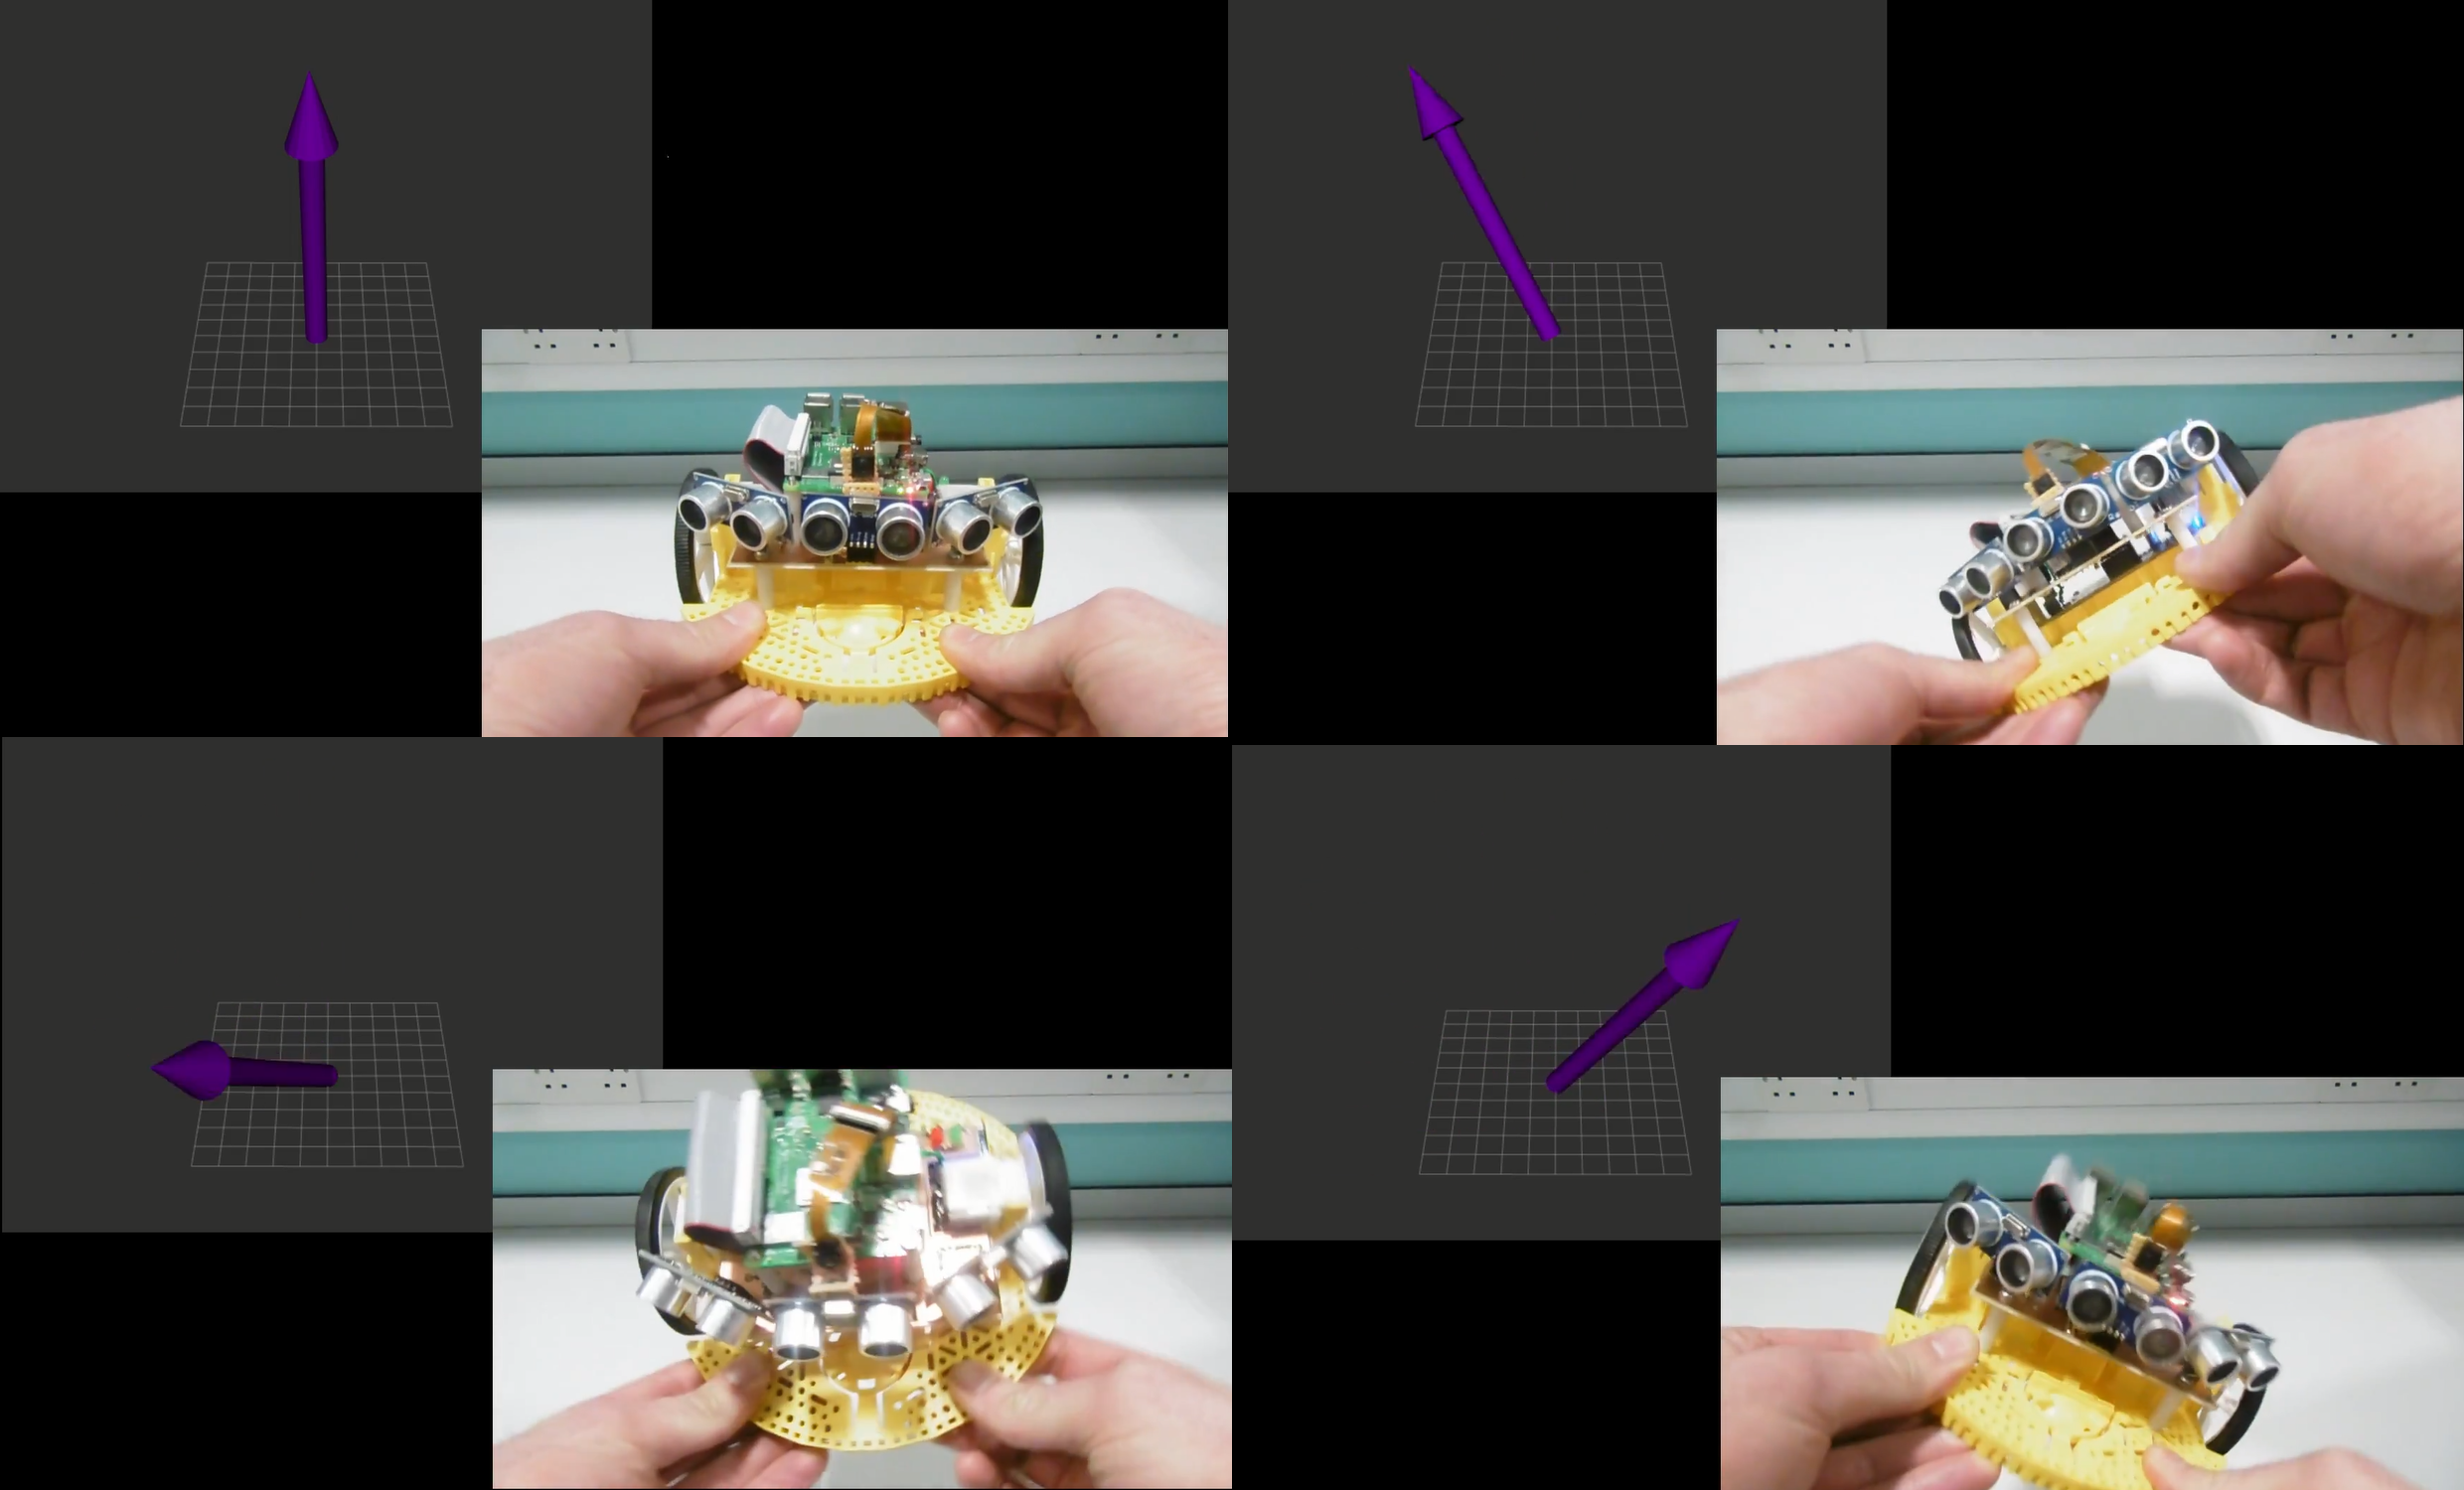
\includegraphics[width=1\textwidth]{IMUtest.png}
	\caption{IMU RVIZ Test}\label{fig:imu_test}
\end{figure}

\subsection{EKF}\label{soft/odometry/test}


\section{SLAM}\label{soft/SLAM}

\subsection{Design}\label{soft/SLAM/design}

\subsection{Implementation}\label{soft/SLAM/impl}

\subsection{Testing}\label{soft/SLAM/test}



\section{Computer Vision}\label{soft/cv}
Computer vision is a very cheap and effective way of gaining a high level 
understanding of the environment. It was used to allow the agents to 
identify other robots and objectives in in the system. Detecting the other 
robots was an essential component to allow communication between robots, 
prevent agents mistakenly mapping other agents,and to recognise when 
ultrasonic interference would occur.

\subsection{Design}\label{soft/cv/design}
The first detection system considered was a CNN, as discussed in Section 
\ref{litreview/cv/objDet/CNN}. This is a very effective system which has 
the advantage of
being able to classify instances of objects that it has not
seen before. This would be essential if the target objects of
the robot was not consistent, for instance if it had to find
people in the search space. This was, however, not essential
in the scope of this project. The major downside to this
system would be the time to implement. To construct a CNN for
this application would require the collection of a large data
set of images of the robots and goals, as well as the time
consuming process of tuning the CNN.

Feature Based Object detection was also considered. As described in 
Section \ref{litreview/cv/objDet/fb}, this only requires a picture to be 
taken of the object and therefore takes far less time to
implement than the CNN solution. However, the accuracy and
consistency are largely dependant on the number of features
detected, and the algorithm's complexity grows relatively
quickly. The basic brute force algorithm involves comparing
every key point in the object image to every key point in the
frame image, which results in an O($n^2$) complexity (although
this can be streamlined, for instance if it becomes impossible
for the distance to be low enough for a pair to be the best
match part way through the distance calculation, it does not
need to be finished). The calculations for deciding the best
outline of the object also become more complicated, as there
will be a lower true positive to false positive ratio as the
best matches (which are found first) are more likely to be
true positives. It was decided that this would be too
computationally intensive considering the strict constraint of
using a Raspberry Pi.

The method used was by far the simplest considered. It identified the other robots and target 
by their colour. This was only possible as each robot used had a distinct coloured chassis, 
which lacks scalability, but was considered an acceptable simplification as this was not the 
focus of the project.

This works by first converting the images from RGB to Hue-Saturation-Value (HSV) colour space, 
simplifying the colour detection as the hue of the pixel is determined by a single value 
instead of the ratio of three values. A colour can then be identified by a range of H values 
and then a minimum S and V values, which is far more intuitive than checking if it falls into a 
range of ratios between R, G and B values.

\subsection{Implementation}\label{soft/cv/impl}
The \textit{vision\_node} works using a ROS spin setup, with a \textit{spin()} function being 
called at a set frequency until ROS closes.

A \textit{RobotDetector} object is declared which has the range of HSV values for each robot 
and the goal, and has a video capture object. It contains a \textit{search()} function which 
takes a frame as a parameter and returns various details about each robot's presence in the 
frame. \textit{search()} first calls \textit{get\_colour\_mask()} for each range of colour 
values. This converts the image to HSV, then makes a frame, \textit{mask}, which is white where 
the pixel in range and and black for out of range. This is shown in Code Listing 
\ref{lst:get_colour_mask}. This also shows the handling of cases where the range of colours 
crosses the zero point (as zero is adjacent to 255 in the hue value).

\begin{lstlisting}[caption={get\_colour\_mask in RobotDetector},label={lst:get_colour_mask} , language=python]

def get_colour_mask(self, frame, lower_hsv_bound, higher_hsv_bound):
        hsv_frame = cv2.cvtColor(frame, cv2.COLOR_BGR2HSV)

        if (lower_hsv_bound[0] > higher_hsv_bound[0]):
            mask1 = cv2.inRange(hsv_frame, np.array([0, lower_hsv_bound[1], lower_hsv_bound[2]]),
                                np.array(higher_hsv_bound))
            mask2 = cv2.inRange(hsv_frame, np.array(lower_hsv_bound),
                                np.array([179, higher_hsv_bound[1], higher_hsv_bound[2]]))
            mask = mask1 | mask2
        else:
            lower = np.array(lower_hsv_bound)
            upper = np.array(higher_hsv_bound)
            mask = cv2.inRange(hsv_frame, lower, upper)

\end{lstlisting}

The function then uses erosion and dilation functions provided by opencv to reduce noise in the 
mask.

The contours in the mask are then iterated through to find the biggest, which is assumed to be 
the object and the centre point and outline of the contour is found. If no contours are bigger 
than a fixed size (measured in pixels) the object is assumed to not be in the image frame, and 
the corresponding \textit{obj\_found} variable is set to false. This process is shown in Code 
Listing \cite{lst:cv_search_loop}.

\begin{lstlisting}[caption={Contour Iteration in search()},label={lst:cv_search_loop} , language=python]
...
for c in contours:
    if cv2.contourArea(c) > max((300, maxsize)):
        maxsize = cv2.contourArea(c)
        cx, cy = self.get_centre_point(c)
        outline = self.get_outline(c)
        obj_found = True
...
\end{lstlisting}

These parameters are then returned to the \textit{\_tick()} function which was called by 
\textit{spin()}. This then renders debug info to the frame if it's performing a test, or 
publishes the detected robot info via a ROS message consisting of a comma separated list of 
objects detected in the last frame.

\subsection{Testing}\label{soft/cv/test}
Initial testing of the \textit{vision\_node} was performed on a PC with a USB webcam. The 
testing was performed by using the position information to render labelled rectangles to a real 
time stream highlighting the position of the objects. The code for this is shown in Code 
Listing \ref{lst:draw_rectangles}.

\begin{lstlisting}[caption={asd},label={lst:draw_rectangles} , language=python]
for i, name in enumerate(names):
    if found[i]:
        #cv2.drawContours(frame, [outline], -1, (0, 255, 0), 2)
        #cv2.circle(frame, (cx, cy), 7, (255, 255, 255), -1)
        x, y, w, h = cv2.boundingRect(outlines[i])
        cv2.rectangle(frame, (x, y), (x + w, y + h), highlight_colours[i], 2)
        cv2.putText(frame, name, (x - 20, y - 20),
                            cv2.FONT_HERSHEY_SIMPLEX, 0.5, highlight_colours[i], 2)
\end{lstlisting}

An example of this running is shown in Figure \ref{fig:cv_screenshot}

\begin{figure}[!ht]
	\centering
	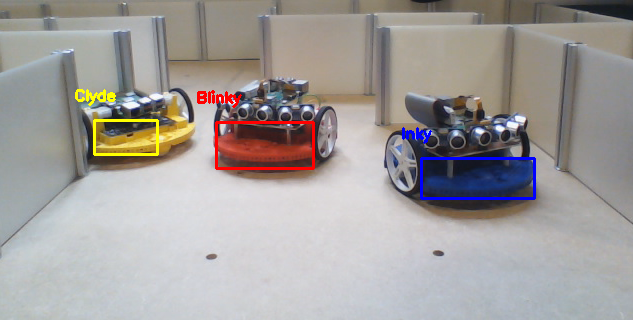
\includegraphics[width=1\textwidth]{ComputerVisionScreenshot.png}
	\caption{Computer Vision PC Test}\label{fig:cv_screenshot}

\end{figure}

The system was then tested on the RPi by monitoring the ROS topic \textit{robots\_detected} to 
test both the integration with the RPi and with ROS. Various detectable objects were moved in 
and out of the frame and changes in the output were observed. This initially failed as the RPi 
camera was connected using a CSI port, not a USB port, which OpenCV's VideoCapture function 
does not support. When running on the RPi, this was replaced with imutil's VideoStream package. 
After this the test performed as expected, consistently identifying which objects were in 
frame.

Functionality was then added to record the feed as to see how the computer vision responded as 
the robot was traversing the maze, however there were issues with frame rate as it was too 
computationally intensive for the RPi to perform the recording as well as all the other 
computation.

\section{AI \& Control Modules}\label{soft/ai}

\subsection{Design}\label{soft/ai/design}

\subsection{Implementation}\label{soft/ai/impl}

\subsection{Testing}\label{soft/ai/test}
